\documentclass[../../main.tex]{subfiles}

Der Fragenkatalog besteht aus folgenden Fragen:
\begin{enumerate}
    \item Was ist dein Lieblings-Videospliel?
    \item Lieber Single- oder Multiplayer?
    \item Was ist dein Lieblingsgenre?
    \item Was ist deine Lieblingskonsole?
    \item Was ist dein Lieblings-Free-To-Play Spiel?
    \item Eigene Konsole mitnehmen / zur Verfügung gestellte verwenden?
    \item Welches Spiel hast du in Quarantäne am meißten gespielt?
    \item Hast du in Quarantäne mehr Single- oder Multiplayerspiele gespielt?
    \item Wie wichtig sind dir Videospiele?
\end{enumerate}

\begin{tikzpicture}
    \begin{axis}[
        title={Was ist dein Lieblings-Videospiel},
        symbolic x coords={
            test,
            my,
            name,
            jeff,
            my2,
            name2,
            jeff2,
        },
        ybar,
        ylabel={Antwortrate [\%]},
        width=\textwidth,
        height=0.4\textheight,
        xtick=data,
        x tick label style={rotate=45,anchor=east},
    ]
        \addplot+[ybar] plot coordinates {
            (test,99)
            (my,22)
            (name,12)
            (jeff,5)
            (name2,12)
            (jeff2,5)
            (my2,50)
        };
    \end{axis}
\end{tikzpicture}